\section{Aut\'omata de Pila}
\subsection{ Descripci\'on del programa}
\justify
El siguiente programa verifica la siguiente gram\'atica $0^n 1^n$ con n $>$0, cuenta con un modo autom\'atico y manual, en la salida se imprimir\'a la historia de la evaluaci\'on de la cadena y si esta es aceptada o no,ademas se guardara de igual forma en un archivo la historia de esta misma evaluaci\'on.\\
El siguiente es un aut\'omata de pila, es decir al recibir un 0 el aut\'omata mete\'ra en la pila una X y al recibir un 1 el aut\'omata sacara esta X. La cadena ser\'a aceptada si la pila se encuentra vacia.\\
\subsection{C\'odigo}
El c\'digo utilizado para la resoluci\'on del problema se muestra a continuaci\'on:\\

C\'odigo:Nodo.java

\lstset{language=Java, breaklines=true, basicstyle=\footnotesize}
\begin{lstlisting}[frame=single]
	
package Stack;


public class Nodo {
    private String dato;
    private Nodo siguiente;

    public Nodo() {
        this.dato="";
        this.siguiente = null;
    }

  
    public String getDato() {
        return dato;
    }

    public void setDato(String dato) {
        this.dato = dato;
    }

    public Nodo getSiguiente() {
        return siguiente;
    }

    public void setSiguiente(Nodo siguiente) {
        this.siguiente = siguiente;
    }
    
    
}

\end{lstlisting}
\vspace{1.5cm}
C\'odigo:Pila.java

\lstset{language=Java, breaklines=true, basicstyle=\footnotesize}
\begin{lstlisting}[frame=single]
	
package Stack;

public class Pila {
    private Nodo tope;

    public Pila() {
        this.tope = null;
    }
    
public void push(String dato){
    Nodo nuevo = new Nodo();
    nuevo.setDato(dato);
    
    if(is_empty()){
        tope=nuevo;
    }
    else{
        nuevo.setSiguiente(tope);
        tope=nuevo;
    }
}
 
public String pop(){
    Nodo auxiliar;
    String dato="";
    if(!is_empty()){
        auxiliar=tope;
        tope=tope.getSiguiente();
        dato=auxiliar.getDato();
        auxiliar=null;
        
    }
    return dato;
}  

public boolean is_empty(){
    if(tope==null){
        return true;
    }
    else{
        return false;
    }
}

    
}

\end{lstlisting}
\vspace{1.5cm}
C\'odigo:AutomataPila.java

\lstset{language=Java, breaklines=true, basicstyle=\footnotesize}
\begin{lstlisting}[frame=single]
	
package automata;

import Stack.Pila;

import java.io.BufferedWriter;
import java.io.File;
import java.io.FileWriter;
import java.io.PrintWriter;


public class AutomataPila {
    private Pila automata;
    private int tamanio;
    private String cadena;
    
    public AutomataPila() {
        automata=new Pila();
       cadena="Z0";
    }
    
    public String evaluar(char caracter,String estado){
        //System.out.println(estado);
        if(estado.equals("q0")){
            if(caracter=='1'){
                if(!automata.is_empty()){
                    estado="q1";
                    automata.pop();
                    cadena=cadena.substring(1);
                    tamanio--;
                }
                else{
                    return "";
                }
            }
            else if(caracter=='0'){
                estado="q0";
                automata.push("X");
                cadena="X"+cadena;
                //System.out.println(automata.imprimirPila());
                tamanio++;
            }
            else{
                return "";
            }
        }
        else if(estado.equals("q1")){
            if(!automata.is_empty()){
                if(caracter=='1'){
                    estado="q1";
                    automata.pop();
                    cadena=cadena.substring(1);
                    tamanio--;
                }
                else if(caracter=='0'){
                    return "";
                }
                else{
                    return "";
                }
            
               }
            else{
                return "";
            }
        }
        return estado;
        }
   
    
    public boolean fin(){
        if(automata.is_empty()){
            return true;
        }
        else{
            return false;
        }
    }
    public void vaciarPila(){
  
        for(int i=0;i<tamanio;i++){
            automata.pop();
        }
        
        }
    
    
   public void IniciarArchivo(String texto){
    File f = new File ("archivo.txt");

        if ( !( f.exists ( ) ) ){
        try {
            FileWriter w = new FileWriter ( f, true );
            f.createNewFile ( );
            w.write (texto);
            } 
        catch ( Exception e ) {
        e.printStackTrace ( );
        }
        } 
        else {
        try{
        FileWriter w = new FileWriter ( f, true );
        w.write (texto);
        w.close ( );
        } 
        
        catch (Exception e ) {
        e.printStackTrace ( );
        }
}
   }
   

    public String getCadena() {
        return cadena;
    }

    public void setCadena(String cadena) {
        this.cadena = cadena;
    }
    
    public int GenerarNumero(){
        int numero;
        numero=(int)(Math.random()*100)+1;
        return numero;
        }
     public int Generarbit(){
        int numero;
        numero=(int)(Math.random()*2);
        return numero;
        }
   
     public String generarCadena(){
     String cadena="";
     int numero=GenerarNumero();
         for (int i = 0; i < numero; i++) {
             cadena=cadena+Generarbit();
         }
     
     return cadena;
     }
}



\end{lstlisting}
\vspace{1.5cm}
C\'odigo:main.java

\lstset{language=Java, breaklines=true, basicstyle=\footnotesize}
\begin{lstlisting}[frame=single]
	
package automata;
import java.util.Scanner;
import javax.swing.JOptionPane;


public class Main {
    
    

    public static void main(String[] args) {
       String cadena;
       String bin_aux;
       String estado="q0";
       char cadena_aux;
       AutomataPila automata=new AutomataPila();
       String opcion;
       String opcion2;
       //Menu
       
       
       System.out.println("Menu\n1.-Modo manual\n2.-Modo Automatico\n3.-Salir\nElija una opcion: ");
       Scanner entrada = new Scanner(System.in);
       opcion=entrada.nextLine();
       
       if(opcion.equals("1")){
           while(true){
                cadena=JOptionPane.showInputDialog(null,"Introduzca una cadena binaria");
                bin_aux=cadena; 
                for(int i=0;i<cadena.length();i++){
                    cadena_aux=cadena.charAt(i);
                    automata.IniciarArchivo("("+estado+", "+bin_aux+", "+automata.getCadena()+")");
                    System.out.println("("+estado+", "+bin_aux+", "+automata.getCadena()+")");
                    estado=automata.evaluar(cadena_aux,estado);
                    
                    bin_aux=bin_aux.substring(1);
                    //System.out.println(estado);
                    if(estado.equals("")){
                        break;
                    }
 
                }
                if(automata.fin() && estado.equals("q1")){
                automata.IniciarArchivo("("+estado+", e ,"+automata.getCadena()+")");
                System.out.println("("+estado+", e ,"+automata.getCadena()+")");
                estado="f";
                automata.IniciarArchivo("("+estado+", e ,"+automata.getCadena()+")\n\n");
                System.out.println("("+estado+", e ,"+automata.getCadena()+")");
                System.out.println("Cadena aceptada");
                }
                else{
                    System.out.println("Cadena no aceptada");
                }
                estado="q0";
                automata.vaciarPila();
                automata.setCadena("Z0");
                while(true){
                System.out.println("Desea evaluar otra cadena\n1.-Si\n2.-No\nElija una opcion: ");
                Scanner rentrada = new Scanner(System.in);
                opcion2=rentrada.nextLine(); 
                if(opcion2.equals("1")){
                    break;
                }
                else if(opcion2.equals("2")){
                    System.exit(0);
                    }
                }        
            }
       }         
       else if(opcion.equals("2")){
           while(true){
                cadena=automata.generarCadena();
                bin_aux=cadena;
                System.out.println(bin_aux);
                for(int i=0;i<cadena.length();i++){
                    cadena_aux=cadena.charAt(i);
                    automata.IniciarArchivo("("+estado+", "+bin_aux+", "+automata.getCadena()+")");
                    System.out.println("("+estado+", "+bin_aux+", "+automata.getCadena()+")");
                    estado=automata.evaluar(cadena_aux,estado);
                    
                    bin_aux=bin_aux.substring(1);
                    //System.out.println(estado);
                    if(estado.equals("")){
                        break;
                    }
 
                }
                if(automata.fin() && estado.equals("q1")){
                automata.IniciarArchivo("("+estado+", e ,"+automata.getCadena()+")");
                System.out.println("("+estado+", e ,"+automata.getCadena()+")");
                estado="f";
                automata.IniciarArchivo("("+estado+", e ,"+automata.getCadena()+")\n\n");
                System.out.println("("+estado+", e ,"+automata.getCadena()+")");
                System.out.println("Cadena aceptada");
                }
                else{
                    System.out.println("Cadena no aceptada");
                }
                estado="q0";
                automata.vaciarPila();
                automata.setCadena("Z0");
                while(true){
                System.out.println("Desea evaluar otra cadena\n1.-Si\n2.-No\nElija una opcion: ");
                int reop=automata.Generarbit();
                    System.out.println(reop+1);
                if(reop==0){
                    break;
                }
                else if(reop==1){
                    System.exit(0);
                    }
                }        
            }
       }
       else if(opcion.equals("3")){
           System.exit(0);
       }
       else{
           System.out.println("Opcion Invalida");
       }
       
       
       
    }
       
      
}

\end{lstlisting}

\newpage

\subsection{Pruebas}
A continuaci\'on se mostraran algunas im\'agenes capturadas al momento de ejecutar el programa, dichas im\'agenes mostraran los resultados obtenidos.\\
\vspace{1.0cm}
Para el modo manual:\\
\begin{figure}[H]
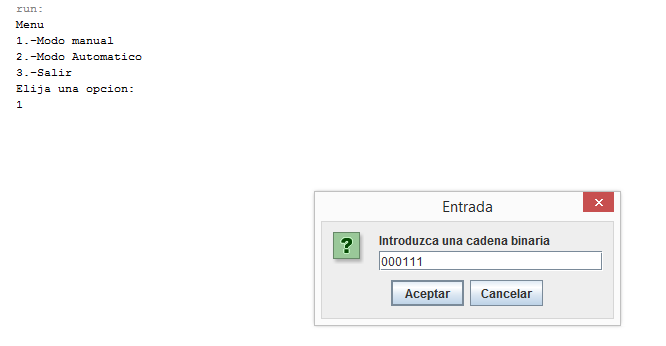
\includegraphics[width=\textwidth, height=7cm]{ModoManualPila.png}
\label{fig:manual_pila}
\caption{Cadena de prueba: 000111}
\end{figure}

\begin{figure}[H]
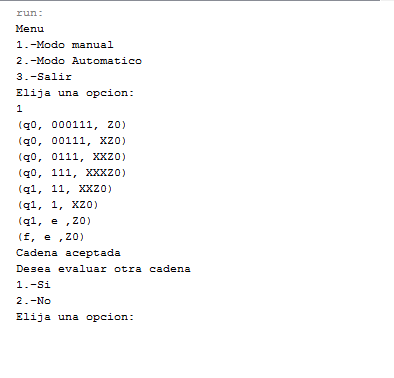
\includegraphics[width=\textwidth, height=7cm]{ModoManualPila2.png}
\label{fig:manual_pila2}
\caption{Cadena de prueba: 000111}
\end{figure}

\begin{figure}[H]
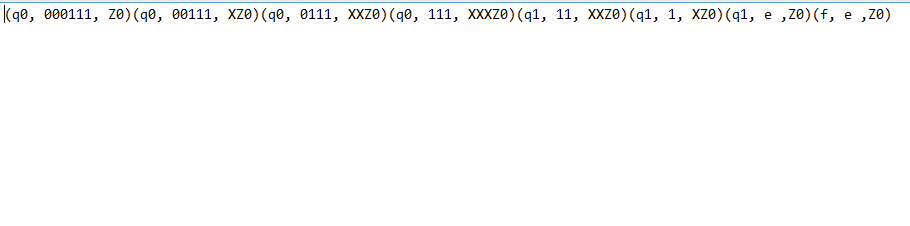
\includegraphics[width=\textwidth, height=7cm]{ArchivoPila.png}
\label{fig:manualtexto_alfabeto}
\caption{Historia de la evaluaci\'on de la cadena}
\end{figure}

Para el modo autom\'atico:\\
\begin{figure}[H]
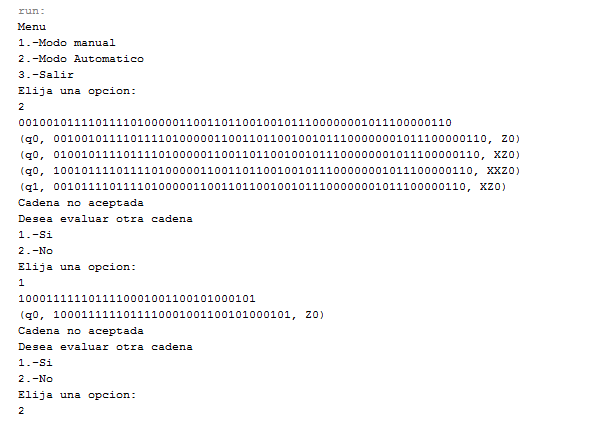
\includegraphics[width=\textwidth, height=7cm]{ModoAutomaticoPila.png}
\label{fig:auto_alfabeto}
\caption{Cadena generada autom\'aticamente}
\end{figure}

\begin{figure}[H]
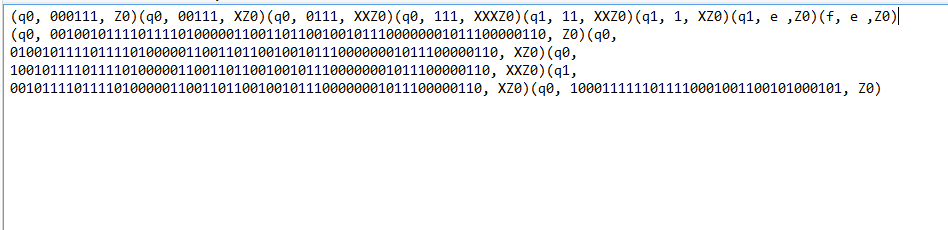
\includegraphics[width=\textwidth, height=7cm]{ArchivoHistoriaPila.png}
\label{fig:autotexto_alfabeto}
\caption{Historia de la evaluaci\'on del modo autom\'atico}
\end{figure}

\newpage
